\begin{figure*}
  \centering
  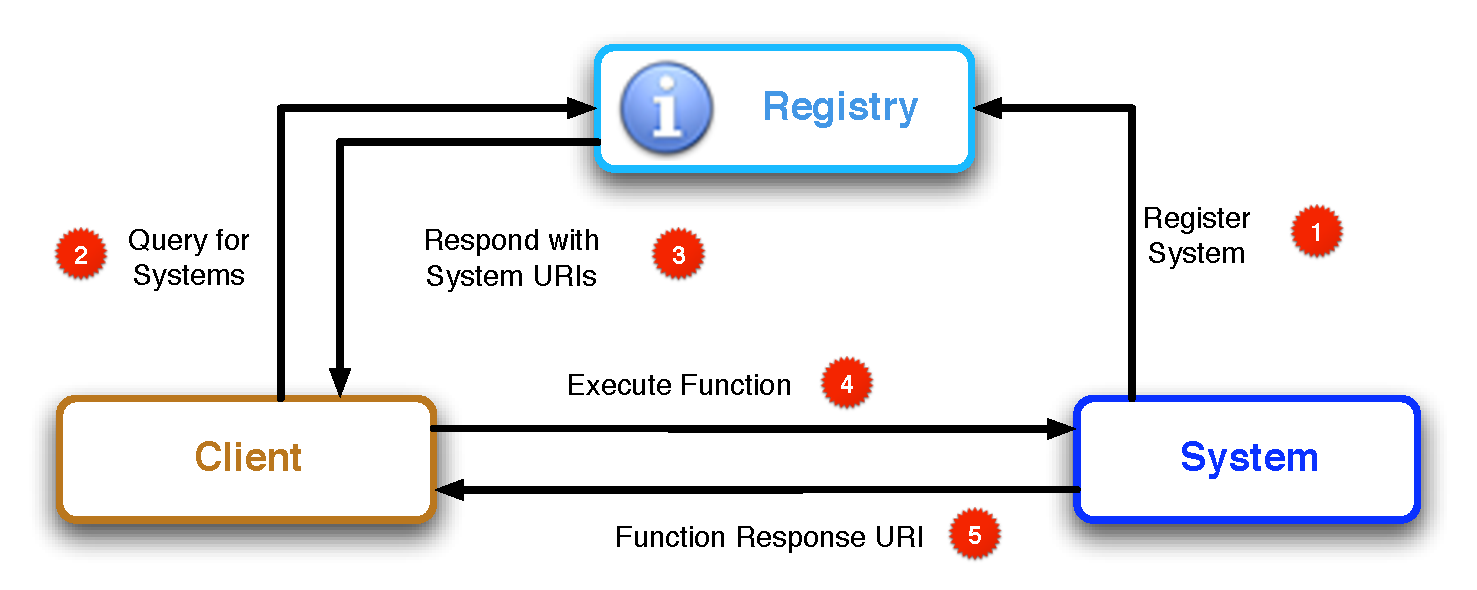
\includegraphics[width=0.70\textwidth]{./images/esp_overview.pdf}
  \caption{ESP framework operations overview.}
  \label{fig:espoverview}
\end{figure*}
\section{System Overview}
The overall architecture for the ESP Framework involves three main components. First, there is the actual system, which represents the sensor network that is being registered. 
The registry is the second element in the architecture and is the location where sensor systems are registered and where the user can actually query for systems.  Finally, there is the
client that accesses both the registry and the individual systems. Figure \ref{fig:espoverview} contains all the entities in the architecture and typical operations that can occur during
normal interaction.

In order to illustrate how the framework works in general, the usage scenarios will be described below.  

\begin{enumerate} \item \textbf{Register System}

During the registration process for a sensor, the first activity that needs to be performed is to create a ESPml document that describes the sensor network system as a whole.  This can be
done manually by an application developer or done automatically by analyzing the sensor system and generating the appropriate XML to represent the
system.  In addition, one must define all the functions that are described as being available in the ESPml document in the actual system.  Finally, the ESPml document must be sent to the
registry.  The process of sending information to the registry occurs through a web services interface where a method for registering the system is exposed.  At the actual registry, the
system ESPml is populated into a database.  More details about the database structure will be given in Section 5.

\item \textbf{Query for Systems}

In order to query for systems, the client sends a request to the registry with an area of interest.  The area is described as a polygon and the actual coordinates are encoded as a ESPml
document.  Again, there is a method exposed on the registry through web services that enables communication between the client and the registry to occur.

\item \textbf{Respond to Query}

After a request for sensor systems is sent, the registry responds to the client by sending back uniform resource identifiers (URIs) for the corresponding systems in the polygon area
submitted.  The actual response is an ESPml document that contains all sensors, platforms, and fields within the polygon. The URIs are addresses to the system's web service interfaces. 
Furthermore, descriptions for the different aspects of the system and the functions provided by these entities are detailed in the ESPml document.

\item \textbf{Function Execution Request}

Once the client gets back all the systems in a certain area of interest, a possible next step is to execute a method on the systems. In this 
case, a light weight version of the ESPml document, which contains only the URIs and the function to execute with any required variables filled in, is sent to the specific system.  
The systems have a web service exposed function to take in generic queries that are defined by the ESPml document.

\item \textbf{Function Response}

The final step in a typical interaction will be the actual system responding to the function execution request.  This occurs by the system returning a ESPml document that contains the
output tag for the function.  The output tag contains the name of the function, the return type for the result, and a URI that points to the result.

\end{enumerate}

Overall, the ESP framework is simple, yet robust enough to handle a wide variety of heterogeneous systems.  Furthermore, the use of ESPml and web services makes interoperable communication
possible in a standard fashion.  More details about each of the different parts of the architecture will be given in Section 5.

